%%%%%%%%%%%%%%%%%%%%%%%%%%%%%%%%%%%%%%%%
% datoteka diploma-vzorec.tex
%
% vzorčna datoteka za pisanje diplomskega dela v formatu LaTeX
% na UL Fakulteti za računalništvo in informatiko
%
% vkup spravil Gašper Fijavž, december 2010
% 
%
%
% verzija 12. februar 2014 (besedilo teme, seznam kratic, popravki Gašper Fijavž)
% verzija 10. marec 2014 (redakcijski popravki Zoran Bosnić)
% verzija 11. marec 2014 (redakcijski popravki Gašper Fijavž)
% verzija 15. april 2014 (pdf/a 1b compliance, not really - just claiming, Damjan Cvetan, Gašper Fijavž)
% verzija 23. april 2014 (privzeto cc licenca)
% verzija 16. september 2014 (odmiki strain od roba)
% verzija 28. oktober 2014 (odstranil vpisno številko)
% verija 5. februar 2015 (Literatura v kazalu, online literatura)
% verzija 25. september 2015 (angl. naslov v izjavi o avtorstvu)
% verzija 26. februar 2016 (UL izjava o avtorstvu)
% verzija 16. april 2016 (odstranjena izjava o avtorstvu)
% verzija 5. junij 2016 (Franc Solina dodal vrstice, ki jih je označil s svojim imenom)


\documentclass[a4paper, 12pt]{book}
%\documentclass[a4paper, 12pt, draft]{book}  Nalogo preverite tudi z opcijo draft, ki vam bo pokazala, katere vrstice so predolge!



\usepackage[utf8x]{inputenc}   % omogoča uporabo slovenskih črk kodiranih v formatu UTF-8
\usepackage[slovene,english]{babel}    % naloži, med drugim, slovenske delilne vzorce
\usepackage[pdftex]{graphicx}  % omogoča vlaganje slik različnih formatov
\usepackage{fancyhdr}          % poskrbi, na primer, za glave strani
\usepackage{amssymb}           % dodatni simboli
\usepackage{amsmath}           % eqref, npr.
%\usepackage{hyperxmp}
\usepackage[hyphens]{url}  % dodal Solina
\usepackage{comment}       % dodal Solina

\usepackage[pdftex, colorlinks=true,
						citecolor=black, filecolor=black, 
						linkcolor=black, urlcolor=black,
						pagebackref=false, 
						pdfproducer={LaTeX}, pdfcreator={LaTeX}, hidelinks]{hyperref}

\usepackage{color}       % dodal Solina
\usepackage{soul}       % dodal Solina

%%%%%%%%%%%%%%%%%%%%%%%%%%%%%%%%%%%%%%%%
%	DIPLOMA INFO
%%%%%%%%%%%%%%%%%%%%%%%%%%%%%%%%%%%%%%%%
\newcommand{\ttitle}{Učenje realno-časovne strateške igre z uporabo globokega spodbujevalnega učenja}
\newcommand{\ttitleEn}{Teaching of real-time strategy game using deep reinforcement learning}
\newcommand{\tsubject}{\ttitle}
\newcommand{\tsubjectEn}{\ttitleEn}
\newcommand{\tauthor}{Jernej Habjan}
\newcommand{\tkeywords}{Alpha Zero, realno-časovna strateška igra, Unreal Engine}
\newcommand{\tkeywordsEn}{Alpha Zero, real-time strategy game, Unreal Engine}


%%%%%%%%%%%%%%%%%%%%%%%%%%%%%%%%%%%%%%%%
%	HYPERREF SETUP
%%%%%%%%%%%%%%%%%%%%%%%%%%%%%%%%%%%%%%%%
\hypersetup{pdftitle={\ttitle}}
\hypersetup{pdfsubject=\ttitleEn}
\hypersetup{pdfauthor={\tauthor, jh0228@student.uni-lj.si}}
\hypersetup{pdfkeywords=\tkeywordsEn}


 


%%%%%%%%%%%%%%%%%%%%%%%%%%%%%%%%%%%%%%%%
% postavitev strani
%%%%%%%%%%%%%%%%%%%%%%%%%%%%%%%%%%%%%%%%  

\addtolength{\marginparwidth}{-20pt} % robovi za tisk
\addtolength{\oddsidemargin}{40pt}
\addtolength{\evensidemargin}{-40pt}

\renewcommand{\baselinestretch}{1.3} % ustrezen razmik med vrsticami
\setlength{\headheight}{15pt}        % potreben prostor na vrhu
\renewcommand{\chaptermark}[1]%
{\markboth{\MakeUppercase{\thechapter.\ #1}}{}} \renewcommand{\sectionmark}[1]%
{\markright{\MakeUppercase{\thesection.\ #1}}} \renewcommand{\headrulewidth}{0.5pt} \renewcommand{\footrulewidth}{0pt}
\fancyhf{}
\fancyhead[LE,RO]{\sl \thepage} 
%\fancyhead[LO]{\sl \rightmark} \fancyhead[RE]{\sl \leftmark}
\fancyhead[RE]{\sc \tauthor}              % dodal Solina
\fancyhead[LO]{\sc Diplomska naloga}     % dodal Solina


\newcommand{\BibTeX}{{\sc Bib}\TeX}

%%%%%%%%%%%%%%%%%%%%%%%%%%%%%%%%%%%%%%%%
% naslovi
%%%%%%%%%%%%%%%%%%%%%%%%%%%%%%%%%%%%%%%%  


\newcommand{\autfont}{\Large}
\newcommand{\titfont}{\LARGE\bf}
\newcommand{\clearemptydoublepage}{\newpage{\pagestyle{empty}\cleardoublepage}}
\setcounter{tocdepth}{1}	      % globina kazala

%%%%%%%%%%%%%%%%%%%%%%%%%%%%%%%%%%%%%%%%
% konstrukti
%%%%%%%%%%%%%%%%%%%%%%%%%%%%%%%%%%%%%%%%  
\newtheorem{izrek}{Izrek}[chapter]
\newtheorem{trditev}{Trditev}[izrek]
\newenvironment{dokaz}{\emph{Dokaz.}\ }{\hspace{\fill}{$\Box$}}

%%%%%%%%%%%%%%%%%%%%%%%%%%%%%%%%%%%%%%%%%%%%%%%%%%%%%%%%%%%%%%%%%%%%%%%%%%%%%%%
%% PDF-A
%%%%%%%%%%%%%%%%%%%%%%%%%%%%%%%%%%%%%%%%%%%%%%%%%%%%%%%%%%%%%%%%%%%%%%%%%%%%%%%


%%%%%%%%%%%%%%%%%%%%%%%%%%%%%%%%%%%%%%%% 
% define medatata
%%%%%%%%%%%%%%%%%%%%%%%%%%%%%%%%%%%%%%%% 
\def\Title{\ttitle}
\def\Author{\tauthor, jh0228@student.uni-lj.si}
\def\Subject{\ttitleEn}
\def\Keywords{\tkeywordsEn}

%%%%%%%%%%%%%%%%%%%%%%%%%%%%%%%%%%%%%%%% 
% \convertDate converts D:20080419103507+02'00' to 2008-04-19T10:35:07+02:00
%%%%%%%%%%%%%%%%%%%%%%%%%%%%%%%%%%%%%%%% 
\def\convertDate{%
    \getYear
}

{\catcode`\D=12
 \gdef\getYear D:#1#2#3#4{\edef\xYear{#1#2#3#4}\getMonth}
}
\def\getMonth#1#2{\edef\xMonth{#1#2}\getDay}
\def\getDay#1#2{\edef\xDay{#1#2}\getHour}
\def\getHour#1#2{\edef\xHour{#1#2}\getMin}
\def\getMin#1#2{\edef\xMin{#1#2}\getSec}
\def\getSec#1#2{\edef\xSec{#1#2}\getTZh}
\def\getTZh +#1#2{\edef\xTZh{#1#2}\getTZm}
\def\getTZm '#1#2'{%
    \edef\xTZm{#1#2}%
    \edef\convDate{\xYear-\xMonth-\xDay T\xHour:\xMin:\xSec+\xTZh:\xTZm}%
}

\expandafter\convertDate\pdfcreationdate 

%%%%%%%%%%%%%%%%%%%%%%%%%%%%%%%%%%%%%%%%
% get pdftex version string
%%%%%%%%%%%%%%%%%%%%%%%%%%%%%%%%%%%%%%%% 
\newcount\countA
\countA=\pdftexversion
\advance \countA by -100
\def\pdftexVersionStr{pdfTeX-1.\the\countA.\pdftexrevision}


%%%%%%%%%%%%%%%%%%%%%%%%%%%%%%%%%%%%%%%%
% XMP data
%%%%%%%%%%%%%%%%%%%%%%%%%%%%%%%%%%%%%%%%  
\usepackage{xmpincl}
\includexmp{pdfa-1b}

%%%%%%%%%%%%%%%%%%%%%%%%%%%%%%%%%%%%%%%%
% pdfInfo
%%%%%%%%%%%%%%%%%%%%%%%%%%%%%%%%%%%%%%%%  
\pdfinfo{%
    /Title    (\ttitle)
    /Author   (\tauthor, damjan@cvetan.si)
    /Subject  (\ttitleEn)
    /Keywords (\tkeywordsEn)
    /ModDate  (\pdfcreationdate)
    /Trapped  /False
}


%%%%%%%%%%%%%%%%%%%%%%%%%%%%%%%%%%%%%%%%%%%%%%%%%%%%%%%%%%%%%%%%%%%%%%%%%%%%%%%
%%%%%%%%%%%%%%%%%%%%%%%%%%%%%%%%%%%%%%%%%%%%%%%%%%%%%%%%%%%%%%%%%%%%%%%%%%%%%%%

\begin{document}
\selectlanguage{slovene}
\frontmatter
\setcounter{page}{1} %
\renewcommand{\thepage}{}       % preprecimo težave s številkami strani v kazalu
\newcommand{\sn}[1]{"`#1"'}                    % dodal Solina (slovenski narekovaji)

%%%%%%%%%%%%%%%%%%%%%%%%%%%%%%%%%%%%%%%%
%naslovnica
 \thispagestyle{empty}%
   \begin{center}
    {\large\sc Univerza v Ljubljani\\%
      Fakulteta za računalništvo in informatiko}%
    \vskip 10em%
    {\autfont \tauthor\par}%
    {\titfont \ttitle \par}%
    {\vskip 3em \textsc{DIPLOMSKO DELO\\[5mm]         % dodal Solina za ostale študijske programe
%    VISOKOŠOLSKI STROKOVNI ŠTUDIJSKI PROGRAM\\ PRVE STOPNJE\\ RAČUNALNIŠTVO IN INFORMATIKA}\par}%
    UNIVERZITETNI  ŠTUDIJSKI PROGRAM\\ PRVE STOPNJE\\ RAČUNALNIŠTVO IN INFORMATIKA}\par}%
%    INTERDISCIPLINARNI UNIVERZITETNI\\ ŠTUDIJSKI PROGRAM PRVE STOPNJE\\ RAČUNALNIŠTVO IN MATEMATIKA}\par}%
%    INTERDISCIPLINARNI UNIVERZITETNI\\ ŠTUDIJSKI PROGRAM PRVE STOPNJE\\ UPRAVNA INFORMATIKA}\par}%
%    INTERDISCIPLINARNI UNIVERZITETNI\\ ŠTUDIJSKI PROGRAM PRVE STOPNJE\\ MULTIMEDIJA}\par}%
    \vfill\null%
    {\large \textsc{Mentor}: doc.\ dr. Matej Guid\par}%
   {\large \textsc{Somentor}:  prof.\ dr. Branko Šter \par}%
    {\vskip 2em \large Ljubljana, 2018 \par}%
\end{center}
% prazna stran
%\clearemptydoublepage      % dodal Solina (izjava o licencah itd. se izpiše na hrbtni strani naslovnice)

%%%%%%%%%%%%%%%%%%%%%%%%%%%%%%%%%%%%%%%%
%copyright stran
\thispagestyle{empty}
\vspace*{8cm}

\noindent
{\sc Copyright}. 
Rezultati diplomske naloge so intelektualna lastnina avtorja in Fakultete za računalništvo in informatiko Univerze v Ljubljani.
Za objavo in koriščenje rezultatov diplomske naloge je potrebno pisno privoljenje avtorja, Fakultete za računalništvo in informatiko ter mentorja.

\begin{center}
\mbox{}\vfill
\emph{Besedilo je oblikovano z urejevalnikom besedil \LaTeX.}
\end{center}
% prazna stran
\clearemptydoublepage

%%%%%%%%%%%%%%%%%%%%%%%%%%%%%%%%%%%%%%%%
% stran 3 med uvodnimi listi
\thispagestyle{empty}
\vspace*{4cm}

\noindent
Fakulteta za računalništvo in informatiko izdaja naslednjo nalogo:
\medskip
\begin{tabbing}
\hspace{32mm}\= \hspace{6cm} \= \kill




Tematika naloge:
\end{tabbing}
Besedilo teme diplomskega dela študent prepiše iz študijskega informacijskega sistema, kamor ga je vnesel mentor. V nekaj stavkih bo opisal, kaj pričakuje od kandidatovega diplomskega dela. Kaj so cilji, kakšne metode uporabiti, morda bo zapisal tudi ključno literaturo.
\vspace{15mm}






\vspace{2cm}

% prazna stran
\clearemptydoublepage

% zahvala
\thispagestyle{empty}\mbox{}\vfill\null\it%
\noindent
Zahvaljujem se mentorju doc.\ dr. Mateju Guidu in somentorju prof.\ dr. Branku Šteru, prijateljem in družini, ki so mi pomagali pri pisanju diplomske naloge.
\rm\normalfont

% prazna stran
\clearemptydoublepage


% kazalo
\pagestyle{empty}
\def\thepage{}% preprecimo tezave s stevilkami strani v kazalu
\tableofcontents{}


% prazna stran
\clearemptydoublepage

%%%%%%%%%%%%%%%%%%%%%%%%%%%%%%%%%%%%%%%%
% seznam kratic

\chapter*{Seznam uporabljenih kratic}  % spremenil Solina, da predolge vrstice ne gredo preko desnega roba

\begin{comment}
\begin{tabular}{l|l|l}
  {\bf kratica} & {\bf angleško} & {\bf slovensko} \\ \hline
  % after \\: \hline or \cline{col1-col2} \cline{col3-col4} ...
  {\bf CA} & classification accuracy & klasifikacijska točnost \\
  {\bf DBMS} & database management system & sistem za upravljanje podatkovnih baz \\
  {\bf SVM} & support vector machine & metoda podpornih vektorjev \\
  \dots & \dots & \dots \\
\end{tabular}
\end{comment}

\noindent\begin{tabular}{p{0.1\textwidth}|p{.4\textwidth}|p{.4\textwidth}}    % po potrebi razširi prvo kolono tabele na račun drugih dveh!
  {\bf kratica} & {\bf angleško}                             & {\bf slovensko} \\ \hline
   {\bf MCTS}      & Monte Carlo tree search               & Monte-Carlo drevesno preiskovanje \\
  {\bf UE4} & game engine Unreal Engine 4 & celostni pogon Unreal Engine 4 \\
  {\bf RTS} & real-time strategy & realno-časovna strateška \\
\end{tabular}


% prazna stran
\clearemptydoublepage

%%%%%%%%%%%%%%%%%%%%%%%%%%%%%%%%%%%%%%%%
% povzetek
\addcontentsline{toc}{chapter}{Povzetek}
\chapter*{Povzetek}

\noindent\textbf{Naslov:} \ttitle
\bigskip

\noindent\textbf{Avtor:} \tauthor
\bigskip

%\noindent\textbf{Povzetek:} 
\noindent 
Z obstoječim Alpha Zero algoritmom smo implementirali učenje in priporočanje akcij v realno-časovni strateški igri.
Pregledali smo krajšo zgodovino globokega spodbujevalnega učenja na igrah in povzeli zakaj je pristop samostojnega učenja najprimernejši.
Za strateško igro smo definirali figure in njihove akcije in zakodirali kompleksno stanje igre s kodirnikom.
Prav tako smo definirali ustavitvene pogoje pri igri, ki nima končnega števila potez na podlagi poškodovanja figur.
Rezultate smo prikazali s Python modulom Pygame in v celostnem pogonu Unreal Engine 4. 
V obeh vizualizacijah lahko igramo proti naučenem modelu, ali pa opazujemo, kako se dva računalniška nasprotnika bojujeta med sabo.
Na koncu smo še pregledali rezultate in povzeli učinek učenja algoritma.
\bigskip

\noindent\textbf{Ključne besede:} \tkeywords.
% prazna stran
\clearemptydoublepage

%%%%%%%%%%%%%%%%%%%%%%%%%%%%%%%%%%%%%%%%
% abstract
\selectlanguage{english}
\addcontentsline{toc}{chapter}{Abstract}
\chapter*{Abstract}

\noindent\textbf{Title:} \ttitleEn
\bigskip

\noindent\textbf{Author:} \tauthor
\bigskip

%\noindent\textbf{Abstract:} 
\noindent With the existing Alpha Zero algorithm, we implemented learning and recommending actions in a real-time strategy game.
We examined the shorter history of deep stimulating learning in games and summarized why the self-learning approach is most appropriate.
For a strategic game, we defined the figures and their actions and encoded the complex state of the game with the encoder.
We also defined the stopping conditions of the game, which has no final number of moves based on damage to the figures.
The results were displayed with the Python Pygame module and the Unreal Engine 4 integrated drive.
In both visualizations we can play against the learned model, or we can observe how two computer opponents are fighting each other.
In the end, we have also reviewed the results and summarized the learning effect of the algorithm.
\bigskip

\noindent\textbf{Keywords:} \tkeywordsEn.
\selectlanguage{slovene}
% prazna stran
\clearemptydoublepage

%%%%%%%%%%%%%%%%%%%%%%%%%%%%%%%%%%%%%%%%
\mainmatter
\setcounter{page}{1}
\pagestyle{fancy}

\chapter{Uvod}


Razvijanje inteligentnega agenta v realno-časovnih oziroma RTS igrah je problem, s katerim se mora soočiti večina razvijalcev teh iger, agentove akcije so pa pogosto predvidljive, saj se človeški igralec nauči njihovih načinov delovanja in jih tako lažje premaga.
Če pustimo agentu, da sam opravlja akcije nekontrolirano, bo izvajal naključne akcije, ki so pa slabše kot vnaprej definirana taktika.
Če pa agentu podamo hevristiko, po kateri se mora ravnati, bo poskušal izvesti čim boljšo akcijo, vendar bo za njen izračun porabil predolgo časa, saj bo moral preiskati cel preiskovalni prostor, ki pa pri realno-časovnih strateških igrah zna biti prevelik.
Na primer 10 enot v igri, kjer ima vsaka 5 možnih potez, se razveji na možen faktor $5^{10}$ ≈ 10 milijonov možnih akcij.
Za igro StarCraft je ocenjenih možnih vsaj $10^{1685}$ možnih akcij, kjer je za šah $10^{47}$ in $10^{171}$ za igro Go~\cite{ontanon2017combinatorial}.

Preiskovanje prostora z grobo silo torej odpade. 
Ostanejo nam potem hevristični algoritmi, kot so Alpha-Beta rezanje ali Monte-Carlo drevesno preiskovanje oziroma MCTS. 
Ampak Alpha-Beta deluje dobro samo pod pogoji, da obstaja zanesljiva evaluacijska funkcija in da ima igra majhen vejitveni prostor, kar je pa lastnost veliko klasičnih namiznih iger kot Go in video iger. Zato se je bolje v takih primerih odločiti za MCTS~\cite{chaslot2008monte}.
MCTS pa ima pomanjkljivost, da si stanj igre ne zapomni skozi več iger, kjer bi lahko to vrednost stanja uporabil za bolj natančen izračun naslednjih stanj.

Za memorizacijo stanj pa pridejo v upoštev globoke nevronske mreže, ki pa z učenjem ugotovijo zakonitosti v učni množici in skozi mnogo iteracij izboljšajo svojo predikcijo določenega izhoda ob določenem vhodu. To je pa točno to, kar potrebuje MCTS kot začetno stanje, iz katerega lažje izračuna najboljšo akcijo.

Da pa nevronska mreža dobi dovolj vhodnih podatkov za učenje, pa moramo realizirati algoritem, ki bo igral proti drugem računalniškem nasprotniku, in pridobil rezultat, ali je to igro zmagal, ali zgubil. 
Ob tem izhodu nevronska mreža nagradi svoje predikcije ob določenem stanju, ali pa jih kaznuje.

To je glavna ideja o implementaciji algoritma, ki jo pa vsebuje algoritem Alpha Zero, ki smo ga uporabili v tej diplomski nalogi.
Algoritem se nauči igranja igre z igranjem iger sam proti sebi, kjer boljša različica algoritma napreduje v naslednji krog.
Ko je model nevronske mreže naučen, ga lahko uporabimo, da nam priporoči akcijo v določenem stanju.
Tako lahko implementiramo računalniškega igralca, ki pridobiva akcije od naučenega modela in jih izvršuje, kot tudi priporočilni sistem za akcije, ki jih prikazujemo človeškemu igralcu. Algoritem nam priporoči akcijo in ne tipa strategije, katerega naj izberemo, kar bi potrebovalo še bolj abstrakten pogled na igro. 

O strateških igrah, njihovih abstrakcijah in zakaj so tako zanimive za raziskovanje umetne inteligence bomo več spoznali v poglavju \ref{chrts}.
V poglavju \ref{alphazero} bomo podrobneje pregledali sestavo Alpha Zero algoritma in zakaj je primeren za našo RTS igro.
Ko bomo imeli sestavljen algoritem, bomo zanj sestavili RTS igro v poglavju \ref{chpravilaigre} in izpostavili, kaj so glavne težave pri takih igrah.
Sestavljen algoritem bomo naučili na igri v poglavju \ref{chucenjemodela}, kjer bomo pregledali razne parametre pri učenju in naučen model potem preizkusili z vizualizacijo v Python modulu Pygame in celostnem pogonu Unreal Engine v poglavju \ref{chvizualizacija}.
Rezulate učenja bomo potem še ocenili in ugotovili, katera vrsta učnih parametrov nam je podala najboljši rezultat v poglavju \ref{chrezultati} in zaključili ugotovitve v poglavju \ref{chzakljucek}.

\chapter{Realno-časovne strateške igre}
\label{chrts}

Realno-časovne strateške igre oziroma RTS igre so žanr strateških iger, kjer igralec nadzoruje množico figur, in poskuša premagati nasprotnika z izgradnjo ekonomije, izboljšavo tehnologije in urjenjem primernih vojaških enot, ki dodajo dodano vrednost k končni zmagi igre. Primer RTS igre je na primer Age of Empires II ali igra StarCraft. 

Izzivi realno-časovnih iger so naslednji:
\begin{itemize}
	\item Upravljanje z viri
	\item Izbira akcij ob nevednosti
	\item Prostorsko in časovno razmišljanje
	\item Sodelovanje med večimi agenti
	\item Modeliranje nasprotnika in učenje
	\item Nesporno načrtovanje v realnem času
\end{itemize}

Zdajšni izzivi:
\begin{itemize}
	\item Planiranje:
	Planiranje v realno-časovni igri je vidno kot več nivojev abstrahiranega stanja igre. Višji kot je nivo, bolj dolgoročni so cilji, kot naprimer gradnja ekonomije, na nižjem nivoju je pa premik posamezne enote ipd.
	\item Učenje:
	Predhodno učenje, ki uporablja posnetke že odigranih iger,
	Učenje v igri, ki uporablja po večini spodbujevalno učenje in modeliranje nasprotnika.
	Učenje med igrami
	\item Negotovost:
	Negotovost nastane zaradi nevidnosti nasprotnika in njegovih potez v vsakem trenutku. Prav tako pa ne vemo akcij, ki jih bo nasprotnik izvedel, zato zgradimo drevo, ki nam pove kaj je najverjetneje da bo nasprotnik naredil.
	\item Prostorsko in časovno razumevanje:
	Prostorsko razumevanje je usmerjeno k postavljanju stavb in pozicijo vojske za obrambo in napad.
	Časovno razumevanje je pa usmerjeno k ugotavljanju, kdaj je primerna izdelava hiš za ekonomijo in kdaj pa za napad.
	\item Izkoriščanje znanja domen:
	Izkoriščanje znanje botov. StarCraft je kompleksen, in to ostaja še odprt problem
	\item Razdelitev nalog~\ref{pic1}:
	Strategija, ki je najvišja abstrakcija (3 min planiranje)
	Taktika, ki je implementacija trenutne strategije (pozicija vojske, hiš - 30 sec planiranje)
	Reakcijska kontrola, ki je implementacija taktike, ki je osredotočena na posamezno enoto
	Analiza terena, ki se osredotoča na strnjena območja in na višinsko prednost
	Pridobivanje znanja, s katerim pridobivamo informacije o taktiki nasprotnika~\cite{survey_real_time_strategy_ai_research_starcraft}.
	
	\begin{figure}[h]
		\begin{center}
			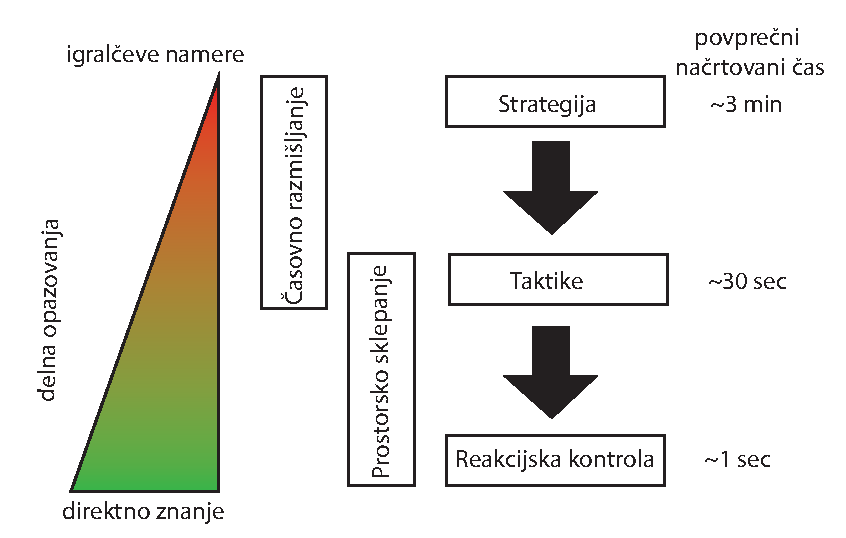
\includegraphics[width=0.6\textwidth]{RazdelitevNalog.pdf}
		\end{center}
		\caption{Razdelitev nalog.}
		\label{pic1}
	\end{figure}
	
	Pogosto razdelimo odločanje na dva dela:
	\begin{itemize}
		\item Micro, kjer kontroliramo enote posamezno
		\item Macro, kjer se osredotočimo na ekonomijo in izdelavo enot
	\end{itemize}
\end{itemize}

\section{Strategija}
V strateških igrah je velikokrat uporabljen pristop direktnega kodiranja strategije, ki uporabljajo avtomate končnih stanj, kjer lahko razbijemo delovanje na več stanj kot so napadanje, nabiranje surovin, popravilo itd. in hitro menjavanje med njimi. Direktno kodiranje prinese dobre pričakovane rezultate, vendar se lahko igralec nauči strategije in ga tako agenta hitro porazi.
Planirani pristopi ponujajo večjo prilagodljivost kot direktno kodirani.
\section{Taktika}
Taktika spada pod direktnejši nadzor enot kakor strategija in je bolj osredotočena na kontrolo določenih točk na mapi, zmagi posameznih bitk in iskanje ožin, kjer je nasprotnik šibkejši. Taktika temelji na analizi terena, ki ga lahko razbijemo na kompozicijo ožin.

\section{Abstrakcija prostora}
Razbiranje strategije in taktike je za algoritme umetne inteligence težji, saj potrebuje višji nivo abstrakcije prostora, figur in akcij, kot za izbiro posameznih nizkonivojskih akcij.

Prav tako problem nastane zaradi negotovosti, kjer ne vidimo nasprotnikovih enot in potez v vsakem trenutku. Predikcija nasprotnikovih potez je tako veliko težja, tako da vsi algoritmi s tako negotovostjo ne delujejo.
Mi smo se za diplomsko nalogo odločili, da imata oba računalniška agenta popoln vpogled na stanje igre in nasprotnikove akcije.

\chapter{Predstavitev algoritma Alpha Zero}
\label{alphazero}
\section{Zgodovina}

Igranje iger je popularno področje znotraj vede o umetni inteligenci. Eden izmed prvih programov je bil programski pogon Checkers (Samuel 2000), ki se je naučil igranja z medotami samo-igranja in strojnega učenja in ne z metodami, ki temeljijo na pravilih.
Leta 2002 je Deep Blue premagal človeškega profesinalnega igralca šaha z nadčloveško sposobnostjo igranja. Pri teh igrah je faktor vejanja akcij še realativno majhen in je lažje oceniti končno pozicijo iz danega stanja.
Rečeno je bilo, da igre kot npr Go, ki imajo toliko večji faktor vejanja $10^{171}$ v primerjavi s šahom, ki pa ima $10^{47}$, ne bo možno ugotoviti vrednost končnega stanja še nekaj desetletij.

Ampak algoritem AlphaGo~\cite{silver2016mastering} je naredil preboj,s tem da uporablja metodo globokega spodbujevalnega učenja in algoritem Monte-Carlo drevesno preiskovanje. Oktobra 2016 je premagal profesionalnega Go igralca na podlagi učenjna na domenskem znanju iger, ki so bile odigrane od ekspertov.Te sistemi so temeljili na predznanju ekspertov za učenje in evaluacijo modela.

Leto za tem, je bil razvit algoritem AlphaGo Zero~\cite{silver2017mastering}, ki opisuje pristop k učenju brez domenskega znanja ekspertov, ampak uporablja metodo samo-igranja. Novi model je prav tako premagal AlphaGo algoritem, kar predstavlja odlične rezultate z vidika, da AlphaGo Zero ne potrebuje človeško usmerjanje pri učenju.

Računalniki se lahko tako naučijo reševanje problema brez človeških ekspertov, ki delajo napake in nimajo takojšnega vpogleda na celotno učno množico, kot to imajo računalniki.

Za tem je bil razvit algoritem Alpha Zero, ki vzame ideje AlphaGo Zero kot temelj, ampak je model generaliziran za poljubne igre, kot na primer šah, Shogi, Go, kjer algoritem potrebuje samo pravila igre, ta pa se uči z globokimi nevronskimi mrežami in tabula rasa algoritmom za spodbujevalno učenje.
Zaradi te generalizacije algoritma, lahko algoritem apliciramo na našo RTS igro, kjer moramo definirati pravila igre.
AlphaZero je drugačen od AlphaGo Zero tako, da AlphaZero vrača rezultate, ki so lahko drugačni od zguba, poraz, kot tudi neodločeno.
Prav tako se razlika pojavi v tem, da so se igre pri algoritmu AlphaGo Zero zgenerirale iz vsej prejšnih iteracij, in se je potem moč modela izračunala proti najboljšim igralcem, medtem ko AlphaZero samo hrani eno nevronsko mrežo, ki se stalno posodablja, namesto da čaga iteracijo da se konča.
\section{Potek učenja}

AlphaZero se uči veretnosti in ocenitve končnega stanja izključno z igranjem proti samemu sebi. 
Te potem uporabi pri preiskovanju z glavno namensko metodo Monte-Carlo drevesnim preiskovanjem, da razišče drevo stanj za akcijo.
Drevo preišče prostor in vrne verjetnost zmage pri izbiri določene akcije iz trenutnega stanja imenovano Pi in oceno končnega stanja iz trenutnega stanja v, ki zavzema vrednosti -1 ali 1 (Poraz, zmaga).
AlphaZero izvede več serij igranja iger proti svojim nasprotnikom, ki predstavlja zdajšni najboljši model igranja.
Rezultat igranja igre je lahko -1 za poraz, +1 za zmago in 0 za neodločeno.
Po vsaki seriji učenja, se izvede proces igranja Arena, kjer oba naučena modela igrata drug proti drugemu nekaj iger, in se na to določi zmagovalen model, ki sedaj postane najboljši model, če je razlika v številu zmag večja za nek faktor. V našem primeru je bil ta faktor 60%.
Parametri nevronske mreže so za tem popravljeni, da minimizirajo napako med predikcijo stanja nevronske mreže in dejanskim rezultatom igre in da maksimizirajo podobnost predikcijo potez nevronske mreže z dejanskimi vrednostnimi akcij, ki jih je vrnil MCTS. Oziroma parametri se nastavijo z gradientnim spustom na funkcijo izgube, ki sešteje napako srednega korena (mean-squared error) in prečne entropije (cross entropy).Nevronska mreža sprejme učne množice stanja iger in vrne ravni vektor predikcije akcij v trenutnem stanju in predikcijo zmage.


\chapter{Definiranje pravil igre}
\label{chpravilaigre}

Igro smo definirali po Surag Nairjevi predlogi za Alpha Zero, ki je na voljo na (portalu?) Github (Insert reference here).
Igra je dodana kot modul, ki vsebuje definicijo igre in njena pravila, igralce, vizualizacijo in izgradnjo modela

Igra je definirana v kvadratni mreži 8x8, kjer polje lahko vsebuje največ eno figuro.
Ostale igre, ki so napisane za to različico Alpha Zero izvedbe, kot na primer štiri v vrsto, gobang, othello, tri v vrsto, vsebujejo črno-bele figure.
Zakodirane so lahko z eno številko: -1 za igralca -1, +1 za igralca +1 ali 0, če je polje prazno.
Pri teh igrah je dimenzija kodiranja 2-dimenzionalna, kjer dimenzije predstavljajo višino in širino igralne plošče.
Pri rts igrah pa moramo vedeti poleg igralca, komur ta figura pripada, tudi stanje te figure, na primer trenutno zdravje in tip figure.
Zato je prostor kodiranja 3-dimenzionalen, kjer je tretja dimenzija zakodirano stanje figure.
Če bi dovolili, da na posamezno polje spada več figur, se dimenzija ponovno poveča za 1.

\section{Definiranje stanja igre}
V tem razdelku smo opisali zapis posamezne figure, njihove akcije in kaj naredijo in tip kodiranja stanja igre, ki ga potem sprejme nevronska mreža.

Sprva moramo definirati figure, ki bodo imele določeno vlogo v igri. Nabor figur je majhen, saj nočemo, da preiskovalni prostor postane prehitro prevelik.
\begin{itemize}
	\item Zlato - Vir surovin, ki predstavljajo denar v igri, s katerim lahko igralec gradi nove stavbe in uri nove enote
	\item Delavec - Figura namenjena gradnji hiš in nabiranju zlata
	\item Vojašnica - Stavba namenjena urjenju vojaških enot
	\item Vojak - Figura namenjena napadanju sovražnikovih enot
	\item Glavna hiša - Stavba namenjena urjenju delavcev in vračanju surovin zlata.
\end{itemize}


Realizirali smo atribute figur. Pomembno je, da so te atributi numerični, da lahko podamo stanje igre kot N-dimenzionalen vektor, ki ga nevronska mreža lahko sprejme in se iz teh numeričnih podakov uči.
Prav tako je pomembno, da ima vsako polje na šahovnici enako število atributov, tudi če je to polje prazno.
Vsako prazno polje ima vanj vpisan atribut čas igranja, ki je splošen za celo igro, vsa ostala polja pa imajo vrednost 0.
\begin{itemize}
	\item Ime igralca: Določa igralca, h kateremu ta figura pripada. Igralec lahko nadzoruje samo svoje figure, izvaja akcije na svojih enotah in napada sovražnikove enote.
	\item Tip figure: Atribut predstavlja numerično predstavitev tipa figure kot naprimer zlato, delavec ipd. Stanje igre potrebuje zapise tipov figur na poljih, da program ve, katere akcije tem figuram pripadajo
	\item Trenutno zdravje: Koliko zdravja ima trenutna figura. Zdravje se lahko povečuje do nekega maksimuma z akcijo zdravi in znižuje z napadom enote
	\item Nosi zlato: Poseben atribut za delavce, ki predstavlja vrednost 1, če figura nosi zlato in 0, če ga ne nosi. To se upošteva pri nabiranju in vračanju zlata, kjer se ti dve akcije ne zgodita v roku ene poteze, ampak se mora stanje prenašati skozi več potez
	\item Denar: Trenutna količina zbranega denarja za posameznega igralca. To polje se ob spremembi količine denarja spremeni v vseh figurah tega igralca
	\item Čas igranja: To polje predstavlja koliko potez se je v trenutni igri že izvedlo. Atribut je prisoten v vseh poljih in se spremeni v vseh poljih šahovnice, ko se izvede nova akcija
\end{itemize}
Poseben primer je figura Zlato, ki ne pripada nobenemu igralcu v večini RTS igrah. V tem primeru pa sem podal vsakemu igralcu svoje polje zlata, da je igra simetrična in nevronska mreža ne interpretira prazno polje igralca kot prazno polje. Prav tako se figuri zlato ne spreminja atribut zdravja, saj jo ne moremo poškodovati. 

\section{Akcije}
Prav tako moramo definirati akcije, ki jih te figure lahko izvajajo. Vsaka figura ne more izvajati vseh akcij, kot naprimer stavbe se ne morejo premikati, same enote kot delavec in vojak pa ne morejo uriti novih enot ~\ref{tabelfigures}.

\begin{itemize}
	\item Nedejaven - Če igralec izbere akcijo nedejavnosti, se ne izvede nobena akcija in se poteza ta igralca zaključi 
	\item Premik gor - Enoti vojak in delavec se lahko premakneta za eno polje proti zgornjemu robu šahovnice če je to mesto prazno
	\item Premik dol  - Enoti vojak in delavec se lahko premakneta za eno polje proti spodnjemu robu šahovnice če je to mesto prazno
	\item Premik levo - Enoti vojak in delavec se lahko premakneta za eno polje proti levem robu šahovnice če je to mesto prazno
	\item Premik desno - Enoti vojak in delavec se lahko premakneta za eno polje proti desnem robu šahovnice če je to mesto prazno
	\item Naberi zlato - Delavec lahko nabere zlato če je v neposredni bližini enote zlato in jih za trenuten čas drži pri sebi 
	\item Vrni zlato - Delavec vrne zlato, ki jih drži pri sebi v glavno hišo, na kar se igralcu prišteje denar
	\item Napadi - Vojak lahko napade sovražno enoto, če je ta v neposredni bližini in jo rani za določen faktor
	\item Izuri delavca - Glavna hiša lahko izuri novo enoto delavec, če ima dovolj denarja, na kar se igralcu odšteje denar
	\item Izuri vojaka - Vojašnica lahko izuri novo enoto vojak, če ima dovolj denarja, na kar se igralcu odšteje denar
	\item Izgradi vojašnico - Delavec lahko izgradi vojašnico na prazno mesto zraven njega, na kar se igralcu odšteje denar
	\item Izgradi glavno hišo - Delavec lahko izgradi glavno hišo na prazno mesto zraven njega, na kar se igralcu odšteje denar
\end{itemize}

Naslednje akcije se izvedejo po nekem zaporedju:
\begin{itemize}
	\item naberi zlato
	\item vrni zlato
	\item napadi
	\item delavec
	\item vojak, 
	\item vojašnica
	\item glavna hiša
\end{itemize}
\begin{verbatim}
coords = [(x - 1, y + 1),
          (x, y + 1),
          (x + 1, y + 1),
          (x - 1, y),
          (x + 1, y),
          (x - 1, y - 1),
          (x, y - 1),
          (x + 1, y - 1)]
for n_x, n_y in coords:
    # check action condition or execute action
\end{verbatim}
Ko je doseženo prvo prazno polje v tem zaporedju, se tam izgradi nova hiša ali izuri nova enota.
Ko je prva sovražna enota izbrana v tem zaporedju, je napadena.
Rezultat tega je gradnja hiš in urjenja enot v spodnji levi kot šahovnice, saj so izbrana prva polja v zaporedju, kot naprimer x-1, y+1, in širjenje proti zgornjim desnim kotom, ko so vsa ostala polja zasedena, oziroma tam ni sovražnih enot.

Popravek za to bi bilo definiranje zgornjih navedenih akcij za vsako izmed teh polj, kar bi se prevedlo v veliko večji prostor akcij.

\section{Kodiranja}

Definirali smo figure, njihove atribute in akcije. Tu so še opisane figure z njihovimi akcijami in nastavljenimi atributi
\begin{table}
\label{tabelfigures}
	\begin{center}
		
	\begin{tabular}{p{0.2\linewidth}|p{0.4\linewidth}|p{0.2\linewidth}|p{0.2\linewidth}}
		Ime figure & {\tt Akcije} & {\tt Zdravje} & {\tt Strošek izdelave} \\ \hline
		{\tt Zlato} & / & 10 & 0 \\
		{\tt Delavec}   & gor, dol levo desno, vojašnica, glavna hiša, naberi zlato, vrni zlato, zdravi & 10  & 1 \\
		{\tt Vojašnica}   & vojak, zdravi & 10  & 4 \\
		{\tt Vojak}   & gor, dol, levo, desno, napad, zdravi  & 20 & 2 \\
		{\tt Glavna hiša}   & delavec, zdravi & 30  & 7 \\
	\end{tabular}


	\end{center}
	\caption{}
	\label{tbl:1}
\end{table}

Definirali smo še začetno stanje vsake igre, kjer sta igralca postavljena v sredino mreže z njihovima glavnima hišama, zraven njiju pa ima vsak igralec svoje polje zlata. Vsakemu igralcu se doda na začetku določena količina denarja za izgradnjo začetnih delavcev. V našem primeru je bilo to 1, tako da je lahko izgradil samo enega delavca.

Sedaj pa potrebujemo zakodirati to stanje igre, v numerični prikaz, ki ga bo nevronska mreža lahko interpretirala. To stanje lahko zakodiramo z desetiškim kodiranjem, vendar obstja možnost, da nevronska mreža sloni proti boljšim obravnavanjem pozitivnih števil za igralca +1, kot za igralca -1. Ravno iz tega razloga obstaja kodiranje One hot, ki spremeni desetiška števila v binarni vektor.

\subsection{Desetiško kodiranje}
Pri desetiškim kodiranjem, predstavimo vsak atribut figure z eno desetiško številko.
Ker imamo figure s 6 atributi, lahko stanje zakodirane igre predstavimo z dimenzijami širina x višina x 6.

Igralec predstavlja številko -1 za igralca -1, 1 za igralca 1 in 0 za prazno polje.


\subsection{One Hot kodiranje}
\begin{itemize}
	\item Ime igralca: 2 bita zaradi treh različnih možnosti: 00 predstavlja prazno polje, 01 predstavlja igralca 1 in 10 igralca -1,
	\item Tip figure: 3 biti, saj imamo 5 različnih figur,
	\item Trenutno zdravje figure: 5 bitov saj hočemo predstaviti večjo številko, zaradi odštevanja zdravja z ranjujočo funkcijo~\ref{destroy_formula_2018_10_20},
	\item Nosi zlato: 1 bit, kjer vrednost lahko zajema vrednost nosi - 1 ali ne nosi - 0,
	\item Denar: 5 bitov, kjer pustimo da igralec gradi ekonomijo in shranjuje denar, da ga potem lahko na hitro zapravi na enotah, ko ga ima dovolj za njihovo izgradnjo.
	\item Čas igranja: $2^{11}$ = 2048, kar pusti igralcu dovolj časa da odkriva nove poteze, ampak ga dovolj hitro omeji, da se konča igra in začne nova
\end{itemize}
Dimenzija zakodiranega prostora je tako 8x8x22

\section{Konec igre}

Konec igre se izvede pod določenimi pogoji:
\begin{itemize}
	\item Igralec nima za izvesti več nobene možne akcije
	\item Vse figure igralca so uničene
	\item Ko se čas izteče
\end{itemize}


\subsection{Reševanje problema neskončnega števila potez}
Čakanje, da se čas igre izteče, je problematično, saj učenje modela poteka zelo počasi, še posebej ko MCTS raziskuje prostor.
Za to smo razvili funkcijo, ki prisili model k izvajanju akcij v zgodnem času igre, drugače figure začnejo pridobivati preveč škode in so zato emilinirane s šahovnice.


\begin{figure}[h]
	\begin{center}
		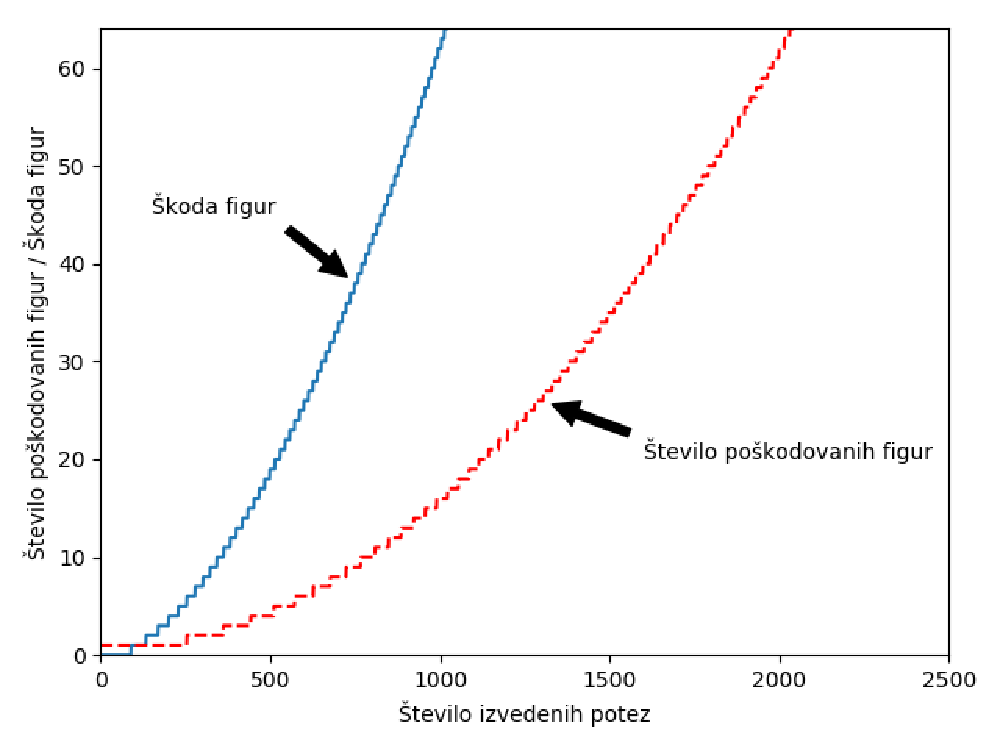
\includegraphics[width=0.8\textwidth]{destroy_formula_2018_10_20.pdf}
	\end{center}
	\caption{Na grafu sta narisani dve funkciji, ki določata škodo, ki se pripeti figuram konec vsake poteze(modra) in število, koliko figur od trenutnega igralca naj se poškoduje(rdeča).}
	\label{destroy_formula_2018_10_20}
\end{figure}

(((((((Modra krivulja predstavlja, koliko škode se obravnava v določeni enoti v danem času igre. Rdeča krivulja predstavlja, koliko igralcev je bilo poškodovanih v trenutnem časovnem okviru.

Vidimo, da je krivulja škode veliko bolj stroga in se v igri začenja že zelo zgodaj. To je zato, ker želimo hitro odpraviti primere, ki ne delajo igralcev, in prednostnim nalogam tistih, ki zbirajo minerale in pridobivajo nove akterje. Vidimo tudi y osi od 0 do 64, kar je največje število igralcev za enega igralca, tako da bo v okolju ~ 8000 vsak igralec na krovu dobil smrtno poškodbo, zato časovni potek nikoli ni dosežen.

Igralci se lahko med seboj zdravijo tudi z denarjem, tako da lahko podaljšajo svoje življenje.)))))))

Blue curve represents how much damage is dealt to specific unit in given game time. Red curve represents how many actors have been damaged in current time frame.

We can see that Damage curve is far more strict and is beginning to rise quite early in the game. That's because we want to quickly eliminate non-working player instances and prioritize those that are collecting minerals and spawning new actors. We can also see y axis span from 0 to 64, which is maximum total of actors for one player, so at round ~8000, every actor on board will recieve fatal damage, so timeout is never reached.

Actors can also heal each other using money, so they can prolong their life.


\chapter{Učenje modela}
\label{chucenjemodela}

(((((Učenje te igre je zapleteno zaradi pogojev končne igre. Učiteljski ovitki pričakujejo, da se igra konča z uporabo simulacij MCTS, vendar pa lahko python zažene v največjo globino rekurzije, če je igralec večkrat ponovil isto potezo.
To se lahko reši z uporabo časovnih omejitev, kjer se simulacija ustavi, ko zmanjkujemo preostalih premikov, vendar lahko povzroči netočno drevo MCTS, ker vozlišča niso pravilno ovrednotena med backpropagation.
Treba je najti ustrezno končno stanje ali spremeniti vir, da izključite časovne omejitve, ker ne vrnejo najboljših rezultatov.


Možna učna ideja
Ideja je, da se s postopnim ucnim modelom spremeni stanje konca igre. Najprej začnite učiti model na preprost način končne igre, kot so izdelava delavcev in ko model uspešno ustvarja delavce, dodajte še en pogoj poleg tega že izvedenega modela.
Možna težava se lahko pojavi zaradi velikosti modela
)))))
Learning of this game is complicated, because of end game conditions. Learning wrapper expects game to finish using MCTS simulations, but python might run into max recursion depth exceeded exception, because player is repeating same move multiple times.
This can be solved using timeouts, as where simulation gets stopped when we run out of remaining moves, but can lead to inaccurate MCTS tree, because nodes do not get properly evaluated during backpropagation.
Proper end condition must be found or change of source is needed in order to exclude timeouts, because they are not returning best resuts.


Possible learning idea
Idea is to incrementally learn model by changing end game condition. First start learning model on simple end game condition like producing workers and when model is successfully creating workers, add another condition on top of that already learnt model.
Possible problem might occur because of model size



\section{TensorFlow}

Keras je module tensorflowa




\begin{izrek}
	\label{iz:1}
	formula po kateri računa verjetnost zmage pri določeni akciji v algoritmu MCTS
	\begin{equation}
	R(s,a) = Q(s,a) + cpuctP(s, a)\sqrt{\dfrac{\sum{b}*N(s,b)}{N(s,a)}}
	\label{eq:1}
	\end{equation}
\end{izrek}

\section{Izbira parametrov}
Cpuct je parameter raziskovanja. V našem primeru je bil nastavljen na vrednost 1.

Pri učenju smo uporabili 

Opišeš parameter mcts sims in cpuct, arenacompare, numiters, numeps, 






\chapter{Vizualizacije}
\label{chvizualizacija}

\section{Pygame}
To je preprosta vizualizacija s Python knjižnico Pygame, za pregled igre med samim razvijanjem. Šahovnica je označena s črtami, med katerimi so s krogi izrisane figure, kjer njihove barve predstavljajo svoj tip enote in obroba krogca igralca -1 ali +1.
V krogcih je tudi napisano zdravje za to enoto in zastavica, ali delavec prenaša zlato.
Zgoraj je izpisano, koliko denarja ima posamezen igralec in koliko potez sta igralca že odigrala. Prav tako so izpisane vse možne akcije, ki jih igralec lahko izvrši z določeno figuro.

Igralec lahko nadzoruje svoje figure s tipkovnico in miško.
Uporabnik mora najprej izbrati figuro z levim miškinim klikom in potem izbrati določeno akcijo, ki je izpisana na zaslonu. Uporabnik lahko spremeni figuro, tako da jo odznači s klikom desnega miškinega gumba na prazno mesto.

\begin{itemize}
	\item Premikanje: igralec lahko premakne delavce in vojake za 1 kvadratek v vseh 4 smereh če so prazni s klikom na eno od 4 mest.
	\item Napadanje: z izbrano vojaško enoto lahko uporabnik napade sovražne enote, ki so v dosegu.
	\item Zbiranje in vračanje sredstev: z izbranim delavcem lahko uporabnik porabi sredstva, tako da klikne desno miškino tipko na polje zlata, če je v dosegu. To velja tudi za vračanje sredstev, vendar mora biti delavec v bližini mestne hiše.
	\item Gradnja: Za gradbene enote in zgradbe mora uporabnik uporabiti eno od bližnjic na tipkovnici.
	\item Nedejaven: igralec lahko z izbranim igralcem pritisne presledek za mirovanje.
\end{itemize}

Prav tako lahko uporabnik igra igro s pisanjem akcij v konzolo.

\begin{figure}[h]
	\begin{center}
		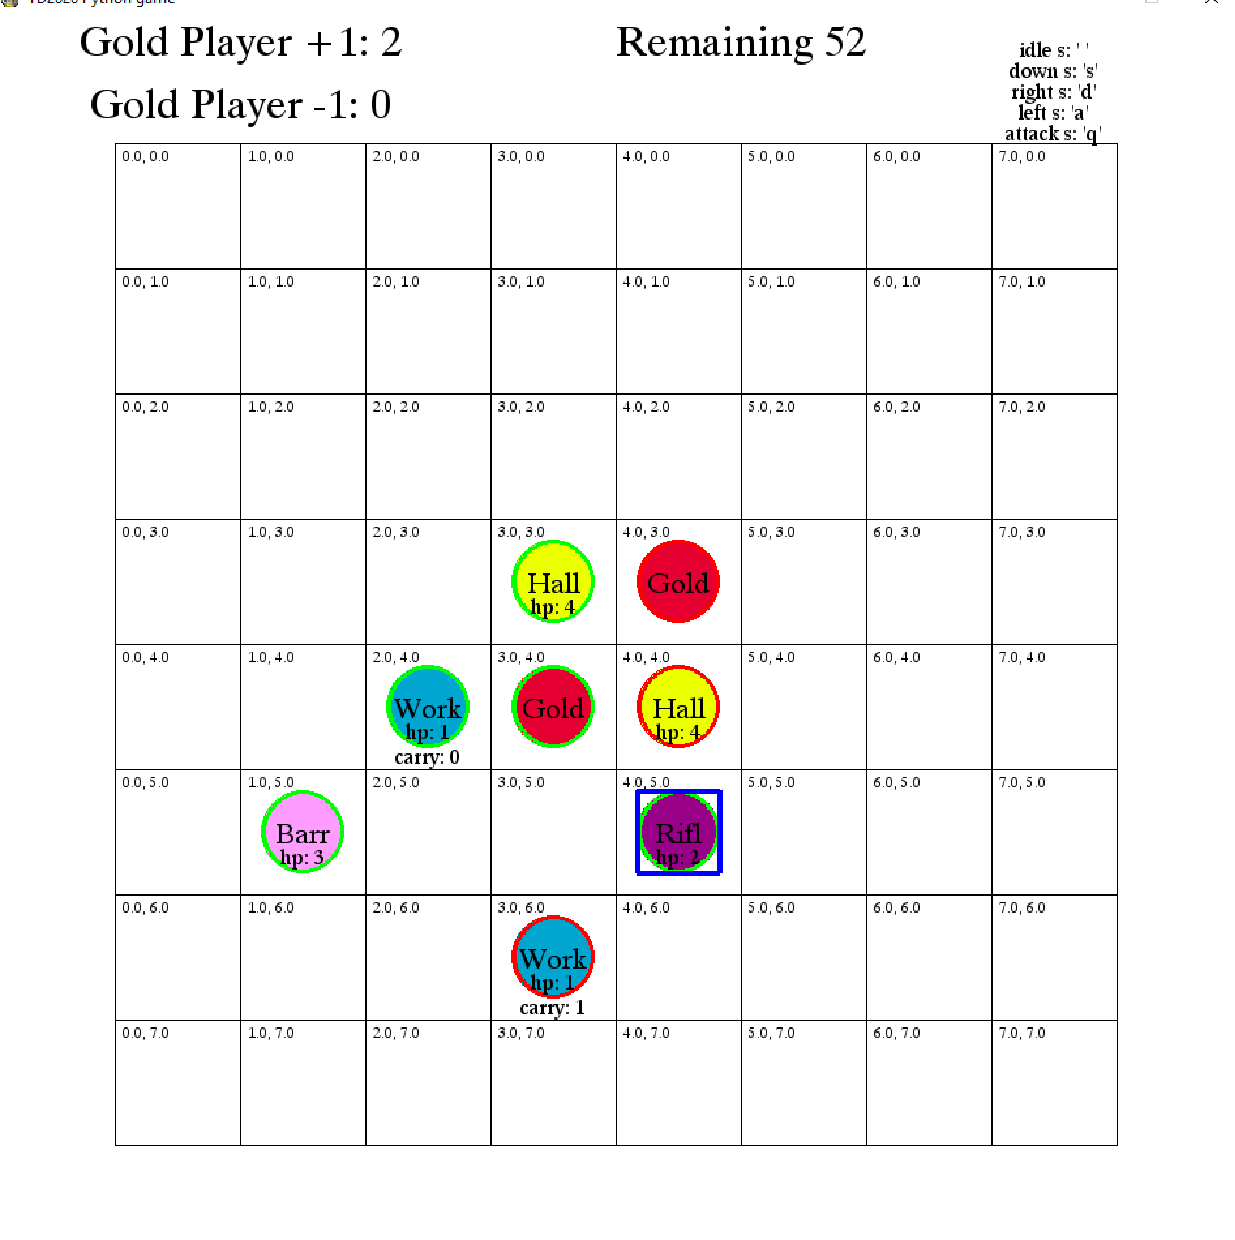
\includegraphics[width=0.8\textwidth]{visualization_pygame.pdf}
	\end{center}
	\caption{Herschelov graf, vektorska grafika.}
	\label{visualization_pygame}
\end{figure}

\section{Unreal Engine 4}

Unreal Engine 4 je odprtokodni program podjetja Epic Games, ki je namenjen hitri izdelavi računalniških iger. Obstajajo še drugi celostni pogoni kot je Unity.\\
Razliko med tema pogonoma je dobro predstavil Marko Kladnik \cite{diploma2}.\\
Unreal Engine 4 omogoča hitro ustvarjanje iger s pomočjo posebnih diagramov (angl. blueprint) in hkrati podpira programski jezik C++, ki ga uporabimo za hitro izvedbo velikega števila matematičnih izrazov.\\

Potrebno je bilo preslikati akcije in figure v urejevalnik Unreal Engine, da se tam enote primerno premikajo in izvajajo akcije.
Potrebno je bilo mapirati animacije, efekte, da premikanje in napadanje zgleda dokaj realistično.

Ta predstavitev omogoča tudi igranje dveh človeških igralcev enega proti drugemu preko internetne mreže, kjer vsak igralec pridobiva priporočene ukaze iz modela.
Človeški igralec lahko igra tudi proti računalniškim igralcem, ki pa vsaki 2 sekundi zahteva za novo najboljšo akcijo.
Lahko si pa ogledamo dva računalniška igralca igrati drug proti drugemu.

\begin{figure}[h]
	\begin{center}
		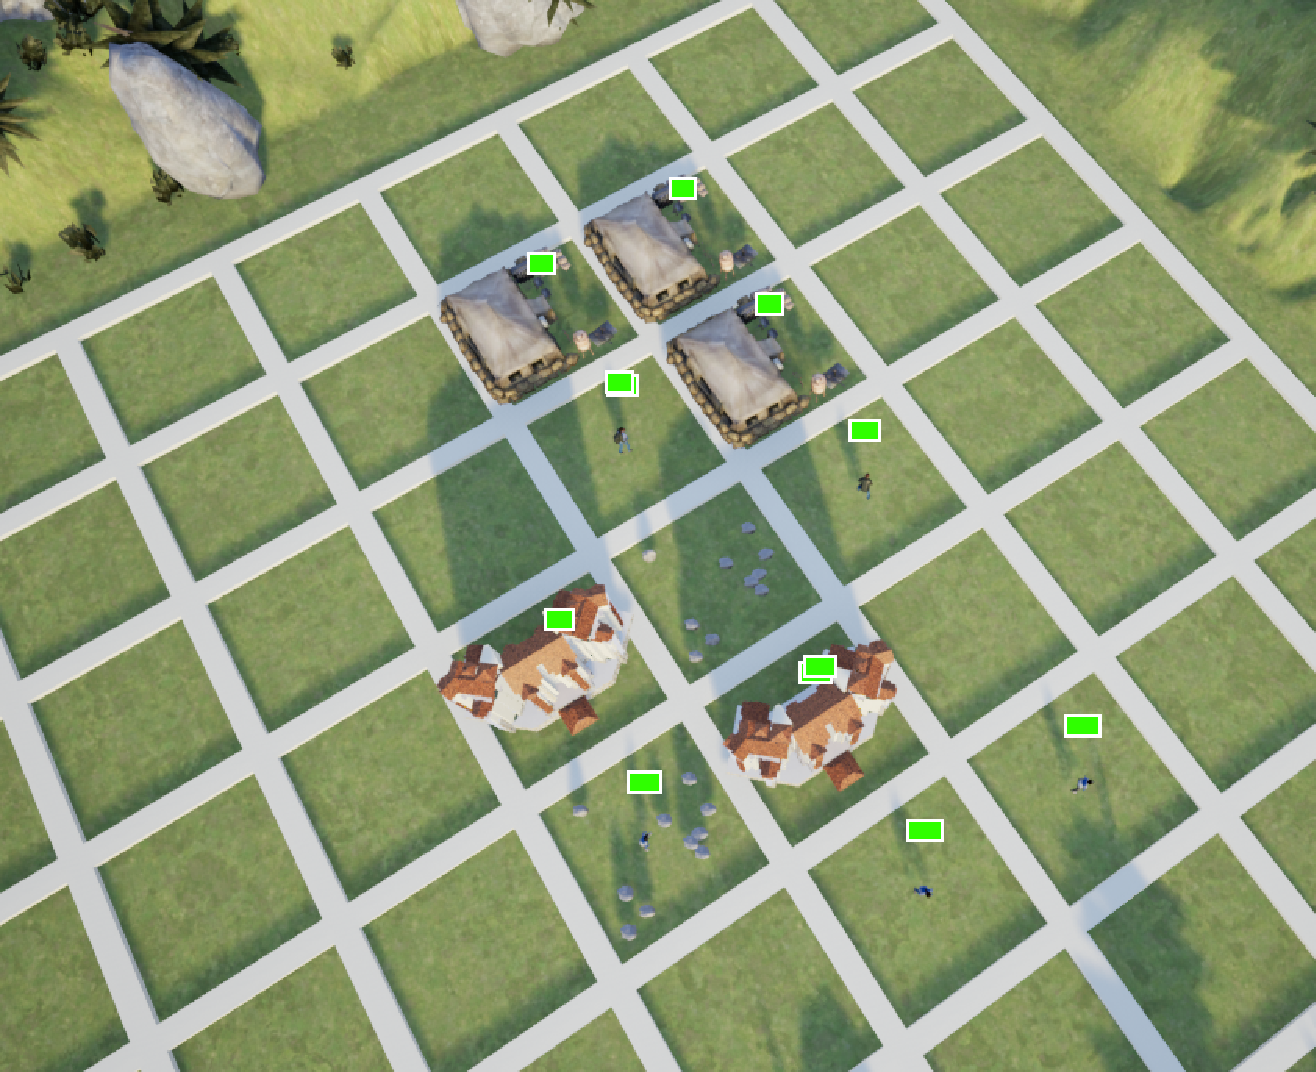
\includegraphics[width=0.8\textwidth]{visualization_ue4.pdf}
	\end{center}
	\caption{Herschelov graf, vektorska grafika.}
	\label{visualization_ue4}
\end{figure}


\subsection{Prenos stanja igre}
napišeš kko encodaš game pa ga pošleš pythonu, tm pa dobiš best action pa pol nazaj...


\chapter{Rezultati}
\label{chrezultati}
Opišeš parametre in čas učenja
Opišeš rezultate pri različnih nastavitvah parametru igre - recmo bolj stroga krivulja, manj stroga, več denarja per mine, cenejši heal...
Pa s kermu encodingom so bli bolši razultati
Pa napišeš primerjava proti naključnim igralcem in greedy- kjer ima greedy player kriterij za število življenja maximize
\section{Izbira ustavitvene funkcije}
Pri izbiri funkcije za timeout smo zelo počasi prišli do dobrih rezultatov.
Pri izbiri ranjujoče funkcije pa smo dobili naslednje rezultate.

\section{Izbira kodiranja}
Pri uporabi desetiškega kodiranja smo dobili naslednje rezultate.
Pri One Hot kodiranju pa smo dobili naslednje rezultate.


\chapter{Zaključek}
\label{chzakljucek}
V zaključku obrazložim ali se algoritem splača vpeljati za moderno RTS igro in kje so vsi problemi.
Opišeš probleme kot so v balanciranju igre, da se nevronska mreža lahko prav nauči in z ugotavljanjem konca igre.

Igra in AlphaZero algoritem je na voljo na naslednjih repozitorijih:\\
https://github.com/JernejHabjan/TrumpDefense2020\\
in \\ 
https://github.com/JernejHabjan/alpha-zero-general


\newpage %dodaj po potrebi, da bo številka strani za Literaturo v Kazalu pravilna!
\ \\
\clearpage
\addcontentsline{toc}{chapter}{Literatura}
\bibliographystyle{plain}
\bibliography{literatura}


\end{document}

